\chapter{Sistemas de Big Data}
\label{chap:bigdata}
Analisando o contexto atual, da nova era da tecnologia, se tem em média 100 bilhões de transações de cartão de crédito por dia acontecendo ao redor do mundo, cerca de 200 milhões de e-mails enviados a cada minuto. Em 2011 a Digital Universe Study (IDC) levantou a seguinte estatística: que a quantidade de dados gerado por mês em 2010 era de 1 exabyte, e ainda projetou que até 2020 esse número cresça 50 vezes mais. Sendo assim a cada dia se produz mais dados de todos os tipos possíveis, estruturados, não estruturados e em diferentes formatos, principalmente após o surgimento do IoT, como já mencionado no capítulo anterior a quantidade de dados gerados por estes dispositivos é imensa. A tabela \ref{tab:medidadados} mostra algumas medidas de dados para comparação com os dados gerado mundialmente.~\cite{sinha2014making}

\begin{table}[h]
\centering
\caption{Grandeza de dados}
\label{tab:medidadados}
\begin{tabular}{|c|c|c|}
\hline 
\rule[-1ex]{0pt}{2.5ex} \textbf{Medida} & \textbf{Representação Numérica} & \textbf{Exemplo} \\ 
\hline 
\rule[-1ex]{0pt}{2.5ex} Byte & 1 & Único caractere \\ 
\hline 
\rule[-1ex]{0pt}{2.5ex} Kilobyte & 1000 & Uma sentença \\ 
\hline 
\rule[-1ex]{0pt}{2.5ex} Megabyte & 1000000 & 20 slides do PowerPoint \\ 
\hline 
\rule[-1ex]{0pt}{2.5ex} Gigabyte & 1000000000 & 10 livros \\ 
\hline 
\rule[-1ex]{0pt}{2.5ex} Terabyte & 1000000000000 & 300 horas de video em boa qualidade \\ 
\hline 
\rule[-1ex]{0pt}{2.5ex} Petabyte & 1000000000000000 & 350 mil fotos digitais \\ 
\hline 
\rule[-1ex]{0pt}{2.5ex} Exabyte & 1000000000000000000 & 100 mil vezes a biblioteca do congresso \\ 
\hline 
\rule[-1ex]{0pt}{2.5ex} Zettabyte & 1000000000000000000000 & Difícil de exemplificar \\ 
\hline 
\end{tabular} 
\end{table}
\legend{Fonte: \citeauthor{sinha2014making}, \citeyear{sinha2014making} (Adaptado)} 

Tendo em vista todos esses dados gerados que até então não serviam para grandes coisas a não ser momentaneamente, eram apenas dados soltos, passou-se a empregar sobre essa massa de dados uma análise, agrupando dados similares, os processando a fim de que através deles fossem possível retirar indicadores, gerar \textit{insights}, criar produtos ou serviços e embasar decisões. É aí que surge o conceito de \textit{Big Data}, que de forma simplista representa uma grande massa de dados, mas está mais relacionado com a grande quantidade e variedade de informações que esta massa de dados pode gerar.~\cite{navegg}

O conceito de \textit{Big Data} ganhou força nos anos 2000, uma época de grandes avanços tecnológicos. Uma aplicação prática de como este conceito pode ser empregado, foi na reeleição de Barack Obama em 2012 para a presidência dos Estados Unidos, quando sua equipe de tecnologia se utilizou do \textit{Big Data} para gerar estatísticas sobre os comentários a respeito do presidente e assim construir estratégias políticas, sendo possível analisar o comportamento de seus eleitores, para que servissem como indicadores de tomadas de decisões políticas pelo presidente.~\cite{sinha2014making}

E este é um dos exemplos mais conhecidos, mas empresas ao redor do mundo tem adotado a implantação de sistemas de \textit{Big Data}, a fim de conhecer o seu público, saber o que os seus clientes estão falando da sua empresa, a fim de buscar informações para o desenvolvimento de novos produtos, tudo isso para alavancar seus lucros, mudando a forma de relacionamento com o cliente e entrega do produto. Esses dados podem ser extraídos de diversos lugares, o Google por exemplo se utiliza da localização GPS das pessoas para que elas avaliem estabelecimentos visitados, para que avisos sobre o trânsito e notícias de interesse por parte do usuário sejam enviados a ele. Desta forma além de benefícios dentro de empresas e governos, o \textit{Big Data} pode trazer também uma melhor qualidade de vida ao usuário, lhe apresentando maiores facilidades no dia a dia, contribuindo com a sustentabilidade e criação de cidades inteligentes.~\cite{navegg}

\section{Gestão dos dados}
\label{sec:gestaodados}
Com relação aos dados que são utilizados para compor o \textit{Big Data}, estes podem ser advindos de diversas fontes e conter os mais variados tipos, podendo ser dados estruturados de forma relacional, documentos de registros de atendimento, fotos, vídeos, que podem ser gerados por máquinas, sensores, humanos, e na sua variedade podem conter dados de mídias sociais, dados gerados por fluxo de cliques de interação em \textit{websites}, dados de localização gerado pelos dispositivos móveis, entre muitas outras fontes que ainda estão por vir.%~\cite{leigos}

O grande desafio tem se tornado agrupar esses dados e encontrar alguma forma com que eles façam sentido, para que a partir de então indicadores capazes de apontar estratégias possam ser gerados. Tendo em vista todos esses dados e a forma com que estão estruturados, nesta nova onda de gestão de dados, é impossível pensar em administrá-los de forma tradicional, para isso foi preciso evoluções não só em software mas também em hardware, além de rede e modelos de computação como virtualização e computação em nuvem. Só desta forma essa massa de dados pôde ser utilizada com maior eficiência.~\cite{leigos}

O \textit{Big Data} não foi algo que surgiu agora, mas foi uma junção dos últimos cinquenta anos de evolução, o que se costuma dividir em três ondas de dados.

\subsection{Primeira Onda}
\label{subsec:primeiraonda}
Em 1960 com a entrada da computação no mercado os dados passaram a ser armazenados em arquivos simples, o que era pouco eficiente, pois para levantar dados sobre clientes era necessário ir em busca de arquivos soltos, em 1970 com a criação do modelo relacional os dados precisaram ser convertidos para esse novo modelo, para isso utilizou-se de força bruta (trabalho manual), pois não havia uma forma de estruturar aqueles dados automaticamente.%~\cite{leigos}

\subsubsection{Modelo Relacional}
\label{subsubsec:modelorelacional}
O Modelo Relacional vem da teoria dos conjuntos (álgebra relacional), representado por um conjunto de tabelas (entidade/relação), estas ainda se dividem em colunas (atributos) e linhas (tuplas), e são nessas tabelas que os dados são armazenados, tendo cada entidade separada em uma tabela, e estas tendo relações entre si através de colunas chaves, desta forma é possível realizar pesquisas em uma entidade isolada ou usar das relações entre elas para se pesquisar mais de uma entidade de única vez.

Quanto a entidade ela é a representação de um componente do mundo real sobre a qual se deseja guardar informações, elas são coisas significativas, como por exemplo: Cliente, Produto e Compra. Desta forma temos entidades que geram valor armazenadas de forma tabular, tendo cada novo registro sendo uma nova linha dentro desta entidade e em cada linha uma sequência de atributos como sendo as colunas, a figura~\ref{fig:modelorelacional} apresenta um exemplo de organização no modelo relacional, com tabelas, atributos e relações.~\cite{relacional}

\begin{figure}[!h]
\caption{\label{fig:modelorelacional} Modelo Relacional}
\begin{center}
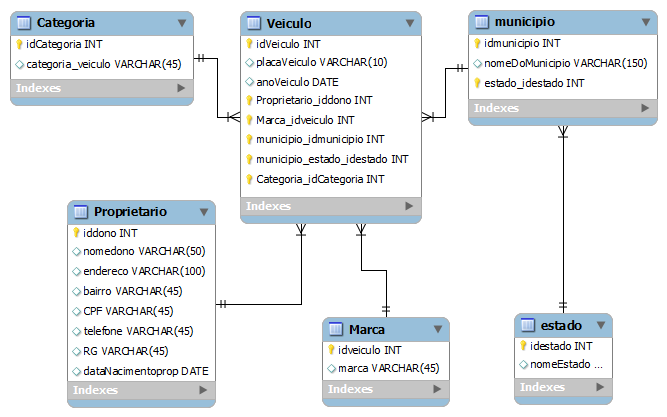
\includegraphics[scale=0.5]{modelorelacional}
\end{center}
%\legend{Fonte: \citeauthor{revistavia}, \citeyear{revistavia}} 
\legend{Fonte: Coelho} 
\end{figure}

\subsubsection{Linguagem SQL}
\label{subsubsec:sql}
Para trabalhar com o modelo relacional foi criado uma linguagem, chamada SQL (\textit{Structured Query Language}), a qual geralmente eram escritas e executadas nos SGBDs (Sistema Gerenciador de Banco de Dados) e tinham a função de manipulação, definição e controle de dados, através de \textit{querys}, que eram sentenças de comandos a fim de realizar uma ação sobre os dados armazenados. Ela mantinha um nível de abstração sobre os dados, além de ser útil para criar relatórios detalhados sobre o cliente, manter um controle de acesso aos dados, e todo o gerenciamento necessário, satisfazendo as exigências crescentes dos negócios. A figura ~\ref{fig:sqlquery} mostra uma \textit{query} escrita em linguagem SQL que busca todos os dados da entidade veículo presente no banco de dados.~\cite{sqlquery}

\begin{figure}[!h]
\caption{\label{fig:sqlquery} \textit{Query} SQL}
\begin{center}
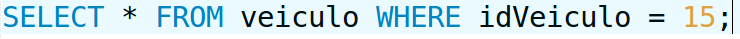
\includegraphics[scale=0.5]{sqlquery}
\end{center}
%\legend{Fonte: \citeauthor{revistavia}, \citeyear{revistavia}} 
\legend{Fonte: Coelho} 
\end{figure}

\subsubsection{Data Warehouse}
\label{subsubsec:datawarehouse}
Com a adoção do modelo relacional, conforme os dados foram crescendo, criou-se em meados da década de 90 o \textit{Data Warehouse} (DW) (armazéns de dados), que é um repositório de dados organizados por assunto, por exemplo em uma empresa de arrecadação de impostos, os assuntos que interessam a empresa são os cadastros de contribuintes e impostos a receber, sendo assim, esses dados são minerados do ambiente transacional da empresa (bancos que estão em produção na empresa), também conhecido como OLTP (\textit{On-line Transaction Processing}), e vão para um DW (um banco a parte) conhecido como OLAP (\textit{On-line Analytical Processing}).

Neste DW é preciso que se tenha integração com a base de dados original, a fim de padronizar os dados que se tem em ambas as bases de dados, é preciso também que ele seja não-volátil, para isso dentro de um DW, só são permitidas operações de consulta e exclusão, mantendo-o não volátil. Outra característica é que ele deve ser variável com o tempo, pois todo dado disponível dentro de um DW se refere a um determinado período de tempo, e esses dados não são atualizados em tempo real para que não afete o desempenho dos bancos transacionais.

Como resultado final de um DW se tem a obtenção de relatórios e estatísticas sobre aqueles determinados assuntos para o qual o DW foi criado, estes são alimentados pelos \textit{Data Marts} que são divisões lógicas dentro do DW, geralmente dentro das empresas é a separação em departamentos, em que cada usuário verá dados relacionados ao seu departamento. A figura \ref{chap:bigdata} mostra a arquitetura básica de um DW.~\cite{datawarehouse}

\begin{figure}[!h]
\caption{\label{fig:sqlquery} Arquitetura de um \textit{Data Warehouse}}
\begin{center}
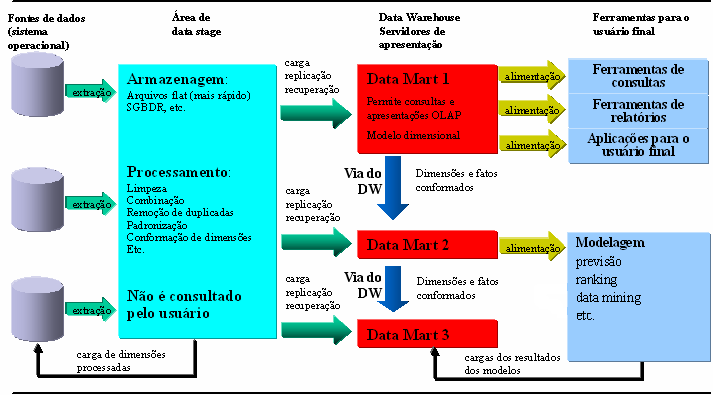
\includegraphics[scale=0.6]{datawarehouse}
\end{center}
\legend{Fonte: \citeauthor{datawarehouse}, \citeyear{datawarehouse}} 
\end{figure}

\subsubsection{Banco de Dados Orientado a Objetos}
\label{subsubsec:bdoo}
Com a popularização de linguagens de programação orientadas a objetos, houve a necessidade de armazena-los da mesma forma com que eram manipulados, sendo assim criou-se o Banco de Dados Orientado a Objetos, uma alternativa ao modelo relacional que se mantêm forte até os dias de hoje. Partindo da premissa de que são armazenados objetos juntamente com seus atributos, mantendo seu estado de quando foram armazenados, o relacionamento entre os objetos se dá da mesma forma que no modelo relacional, se utilizando de chaves estrangeiras, e nas relações de "tabela-filha" neste tipo de armazenamento seria um atributo que tenha como valor outro objeto. Eles são armazenados serializados, sendo possível retornar ao seu estado quando são deserializados.~\cite{bdoo}

\subsection{Segunda Onda}
\label{subsec:segundaonda}
Na década de 1990 com o surgimento da \textit{web}, deixou de se armazenar apenas documentos, para se armazenar áudio e vídeo também, fazendo com que novas tecnologias surgissem para dar conta da nova demanda, criando assim na área da gestão de dados um modelo mais unificado, os metadados.~\cite{leigos}

\subsubsection{Metadados}
\label{subsubsec:metadados}
De forma simplista é possível dizer que metadados são dados que descrevem dados, ou seja ele mantêm uma descrição concisa sobre o tipo do dado armazenado, seja ele tabela, imagem, gráfico ou vídeo. O banco de dados se utilizam de metadados para armazenar o tipo de dado que contêm nas tabelas por exemplo, as classes de objetos são metadados dos objetos, entre muitos outros exemplo. Mas o que é importante destacar é que se os dados não estão documentados, é possível que haja inconsistências, além de maior dificuldade de manutenção desses dados.~\cite{metadados}

\subsection{Terceira Onda}
\label{subsec:terceiraonda}
Na terceira onda está compreendido a era atual, em que a gestão de dados evoluiu para o \textit{Big Data}, fase na qual se tem dados como foto, vídeo e áudio a serem armazenados, desta forma a alternativa encontrada foi virtualizar esses dados e armazená-los em nuvem, pois avanços com relação a velocidade de rede e confiança, removeram muitas limitações físicas da capacidade de administrar quantidades massivas de dados, alinhado com a sofisticação de memórias de computadores, possibilitando assim o avanço para essa nova era.%~\cite{leigos}

Muitas das tecnologias empregadas no \textit{Big Data} existem a anos, como virtualização de dados, processamento paralelo, sistema de arquivos distribuídos e base de dados \textit{in-memory}, mas se tem algumas das tecnologias que foram criadas agora para atender o que o \textit{Big Data} se propõem a entregar, como o Hadoop e MapReduce. Não só na área privada, mas o ramo da ciência, pesquisa e o governo tiveram uma grande parcela no incentivo para o desenvolvimento dessas tecnologias, pois era necessário analisar o genoma humano, analisar os dados astronômicos e coletar dados para fins antiterroristas, o que são alguns dos exemplos de utilização nessas áreas.%~\cite{leigos}

Desta forma \textit{Big Data} não vem a ser uma ferramenta ou tecnologia específica, mas sim um encontro de tecnologias diferentes que quando juntas promovem ideias certas, no tempo certo, baseadas nos dados certos, sejam eles vindos de qualquer fonte geradora de dados. As próximas evoluções tendem a ser através da junção de outras tecnologias que já existem e possam ser utilizadas de alguma forma a integrar com o \textit{Big Data}.~\cite{leigos}

\section{Características do Big Data}
\label{sec:funcbigdata}
Comumente são usadas três características para se descrever o \textit{Big Data}, o que é chamado de 3Vs (volume, velocidade e variedade), ainda existem outras abordagens que tratam como 5Vs (volume, velocidade, variedade, veracidade e valor), estas características mencionadas servem como pré-requisito para se caracterizar armazenamentos e análise de dados como \textit{Big Data}.

\subsection{Volume}
\label{subsec:volume}
A quantificação do volume de dados na computação é relativa, pois ela é dependente do tempo, o que hoje pode ser considerado um volume grande amanhã pode já não ser mais, por esse fato muitas mídias de armazenamento foram sendo substituídas por outras, pois a demanda de armazenamento cresce exponencialmente e novas formas para se armazenar dados precisam ser criadas.~\cite{forbes} 

O \textit{Big Data} tem a proposta de trabalhar com um volume de dados atualmente considerado grande o suficiente para que os modelos tradicionais não suporte o mesmo trabalho, dados como iterações em redes sociais, trocas de email diária, transações bancárias, entre outros. Estes são exemplos de dados hoje considerados muito grandes para se trabalhar de forma tradicional, até porque muitos desses dados não estão estruturados e trabalham com tipos de dados diferentes.~\cite{forbes}  

\subsection{Velocidade}
\label{subsec:velocidade}
\begin{citacao}
Você cruzaria uma rua vendado se a última informação que tivesse fosse uma fotografia tirada do tráfego circulante de 5 minutos atrás? Provavelmente não, pois a fotografia de 5 minutos atrás é irrelevante, você precisa saber das condições atuais para poder cruzar a rua em segurança.~\cite[p. 2]{forbes} 
\end{citacao}

É exatamente isso, nessa nova onda houve uma imersão de tecnologias \textit{real time}, não que antes não existissem, mas com as novas tecnologias seu uso se tornou mais acessível, e para que ela funcione cumprindo seu propósito é necessário que haja velocidade, tanto no armazenamento, como na busca e na analise de resultados. É importante ressaltar que esse conceito de velocidade não está necessariamente relacionado com rapidez, mas sim com a exatidão do tempo de determinada ação, por mais que uma determinada ação demore horas, o importante é ao final desse tempo pré estipulado, o resultado estar disponível.~\cite{forbes} 

\subsection{Variedade}
\label{subsec:variedade}
Quando se fala de variedade dentro de \textit{Big Data}, isto se refere a grande variedade de dados com que ele trabalha, além de virem de fontes diferentes, os mesmos possuem formatos diferentes, organizado em diferentes formas, por exemplo fotos, áudio, vídeo, informações de usuários, todas essas informações estarão organizados de forma estrutural, semi estrutural e não estrutural e o \textit{Big Data} deve ser capaz de trabalhar com eles.~\cite{forbes} 

\subsection{Veracidade}
\label{subsec:veracidade}
Veracidade está diretamente relacionado com a velocidade, pois para os resultados obtidos serem verídicos, ou seja serem confiáveis, é necessário que ele pertença ao tempo que se pretende analisar, de nada vale uma análise de dados que gerou resultados de um tempo passado, é necessário o dado verídico no tempo esperado, caso contrário não será possível se utilizar dos resultados obtidos, por isso a velocidade influencia na veracidade.~\cite{forbes} 

\subsection{Valor}
\label{subsec:valor}
O valor está relacionado ao propósito de se fazer o uso do \textit{Big Data}, pois antes da análise e obtenção de resultados, é necessário que se tenha questionamentos a serem respondidos através do uso do \textit{Big Data}, ou seja, é necessário que o resultado obtido gere valor para o fim que ele está sendo usado, seja ele melhora no relacionamento da empresa com o cliente ou em áreas da ciência ou ainda do governo.~\cite{forbes} 

\section{Processamento de dados em tempo real}
O termo \textit{Big Data}, como já explicado anteriormente, é utilizado quando o grupo de dados que esta sendo analisado é tão grande que não pode ser processado através de técnicas clássicas como utilização de banco de dados relacional (RDBMS ou \textit{Relational Data Base Systems}. E a necessidade de velocidade em toda \textit{pipeline} é acentuada ainda mais quando se pretende fazer processamento em tempo real dos dados obtidos.

Até 2014 uma das mais notáveis ferramentas para o gerenciamento de um grande volume de dados era o MapReduce, uma biblioteca desenvolvida pela Google que oferecia uma grande quantidade de ferramentas em um único pacote para lidar com muitos os desafios que se encontrava em sistemas \textit{Big Data}. Logo após o anúncio do MapReduce pela Google saíram muitas bibliotecas \textit{Open Source} com o mesmo objetivo, entre elas estavam  Hadoop MapReduce e Haddop YARN.

Embora MapReduce faça com que o processamento de larga escala em dados complexos fiquem bem mais simples e eficiente ele ainda se trata de processamento em \textit{batch}, e não era ideal para a demanda recente de processamento em tempo real de um alto volume de dados.

A solução para esse caso pode ser dividida em dois campos, a solução que tenta reduzir o gargalo das tecnologias como MapReduce e fazer com que ele execute seu trabalho mais rápido, e/ou uma segunda solução que provê meios para que as \textit{queries} sejam executada tanto em bando de dados SQL quanto NoSQL.~\cite{realtime}

\subsection{Computação em memoria}

Muitos dos problemas tanto do MapReduce quanto do Hadoop é que seu sistema de processamento em \textit{batch} não era otimizado para uma execução rápida, e sim para processar uma quantidade grande de informação.O Hadoop é muito dependente de um disco rígido para armazenar as informações isso adiciona mais um gargalo para o \textit{startup} de uma tarefa \textit{batch}.

Mesmo que a máquina esteja equipada com vários módulos de I/O, o problema ainda persistirá pois se trata de uma limitação do hardware e qualquer requisição de I/O ainda é muito lenta para operações em tempo real. Uma solução elegante seria armazenar toda a informação em sistemas de memória distribuída.

A memória pode oferecer uma alta quantidade de informação a mais de 10 GB/s. A latência no acesso a informação sendo na casa do nanosegundos enquanto a do disco fica na casa do milissegundo. Combinado com o preço da memória RAM, que vem ficando mais barato, torna o argumento de computação em memória muito mais viável. Há algumas soluções para computação em memória, entre elas estão; Apache Spark, GridGrain e XAP.

Computação em momoria não significa que toda a informação tem que estar na memória, mas se somente uma parte da informação estiver em cache na memória já significaria um grande ganho de performance.~\cite{realtime}

\subsection{Hadoop}
Hadoop em resumo é uma biblioteca para sistemas processamento distribuído de grande quantidade de informação entre \textit{clusters} de computares usando modelos simples de programação. Ele é desenvolvido para escalar de um simples computador para milhares, onde cada um pode oferecer sua própria unidade de computação e armazenamento.~\cite{hadoop}

Hadoop pode resolver diversos problemas no campo de \textit{Big Data} oferecendo velocidade e variedade como discutido nos 5Vs. O fluxo do Haddoop pode ser separado em 4 etapas:~\cite{hadoopessentials}

\begin{itemize}
\item \textbf{Captura dos dados:} as fontes de dados é extensiva e pode ser tando estruturada, semi-estruturada, e até \textit{streaming} de dados (tempo real). Estendendo também para sensores e diversos dispositivos. Tendo integração com diversas fontes de dados como Flume, Storm, e outros fontes de dados do sistema Hadoop.

\item \textbf{Processamento:} se trata de filtros e transformações que serão aplicados  nos dados usando ferramentas baseada na lógica do MapReduce. Hadoop hoje suporta uma quantidade grande de bibliotecas como MapReduce, Hive, Pig, Spark, Storm, etc como mostrado na figura ~\ref{fig:hadoopint}.
	
\begin{figure}[!h]
		\caption{\label{fig:hadoopint} Sistemas que se integram com Hadoop.}
		\begin{center}
			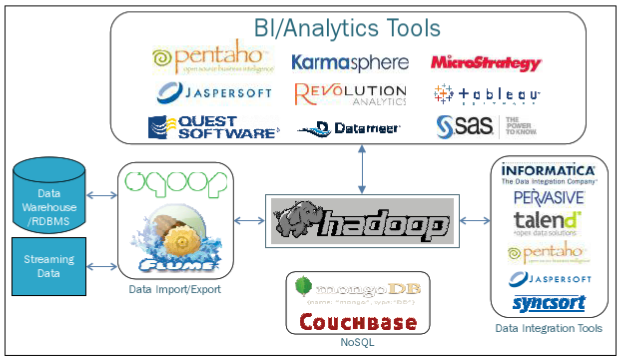
\includegraphics[scale=0.6]{hadoop_int}
		\end{center}
		\legend{Fonte: \citeauthor{hadoopessentials}, \citeyear{hadoopessentials}} 
\end{figure}

\item \textbf{Distribuição:} apos tratamento o dados podem ser distribuído para serem utilizado pela área de BI (\textit{Business Intelligence}), e outros sistemas de analise podem consultar os dados.
	
\item \textbf{\textit{Feedback}}: trata-se de analisar os dados e auditar para futuras melhoras no sistema \textit{Big Data}.
\end{itemize}

A figura ~\ref{fig:hadoopflow} mostra como o dado e capturado e então processado pelo Hadoop, e os resultado são utilizados em sistemas de BI.~\cite{hadoopessentials}

\begin{figure}[!h]
	\caption{\label{fig:hadoopflow} Fluxo básico de informações do Hadoop.}
	\begin{center}
		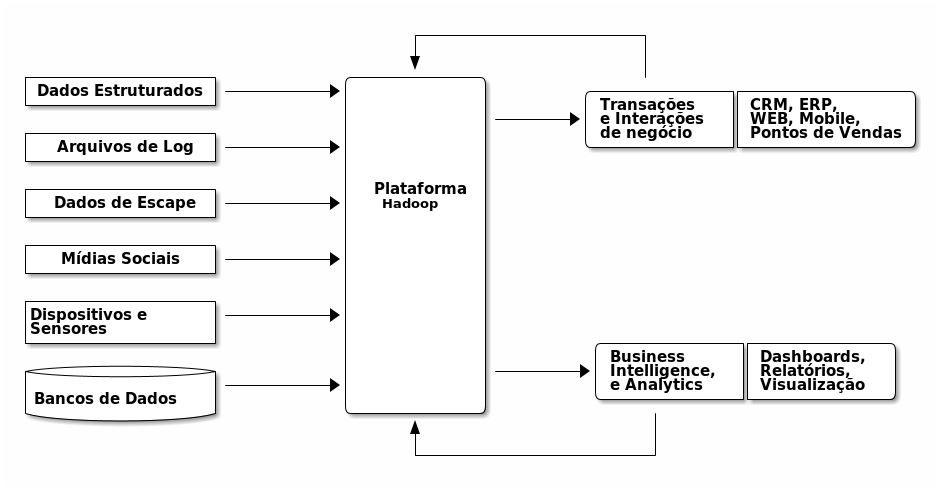
\includegraphics[scale=0.6]{hadoop_flow}
	\end{center}
	\legend{Fonte: \citeauthor{hadoopessentials}, \citeyear{hadoopessentials}} 
\end{figure}


\subsection{Apache Spark}
Apache Spark é um sistema \textit{cluster} de uso geral com foco em velocidade. Ele provê APIs em Java, Scala, Python e R, e um \textit{engine} otimizada que suporta grafos de uso geral. Entres suas bibliotecas ele possui um grupo de ferramentas de alto nível incluindo Spark Sql, MLlib para aprendizado de maquina, GraphX para processamento de grafos e também Spark Streaming para processamento de dados em tempo real.

Abstraindo Spark em um alto nível pode-se dizer que cada aplicação Spark consiste de um \textit{driver} que roda na função principal e executa diversas operações em paralelo em um \textit{cluster}. Spark também provê entre seu grupo de  ferramentas um \textit{resilient distributed dataset}(RDD), que consiste em uma coleção de elementos particionados entre diversos nós de um \textit{cluster}. Esses elementos particionados podem ser acessadas de forma paralela. Normalmente os RDD são criados a partir de um HDFS. Pode-se escolher também hospedar esse RDD em memoria, deixando-o assim mais eficiente.

Uma segunda abstração são as variáveis compartilhadas que podem ser usadas em operações paralelas. Normalmente quando se inicia uma função em paralelo uma cópia das variáveis é usada em cada instância. Mas algumas vezes se quer compartilhar essas informações com todas as tarefas.

\subsubsection{Spark Streaming}
Spark Streaming é uma extensão do \textit{core} do Spark Api que habilita escalabilidade, alta disposição, tolerância a falhas de \textit{data streams}. Dados podem ser utilizados a partir de um grande número de fontes como Kafka, Flume ou até mesmo \textit{sockets} TCP como mostrado na figura~\ref{fig:sparkstreaming}. Esses dados podem ser processados utilizando algoritmos complexos que podem ser expressados em funções de alto nível como \textit{map, reduce, join,} e \textit{window}. Podendo ser aplicados outros algorítimos de aprendizado de máquina e processamento de grafos do próprio ecossistema Spark.~\cite{sparkstreaming}

\begin{figure}[!h]
	\caption{\label{fig:sparkstreaming} Exemplo de fonte de informação que o Spark Streaming suporta.}
	\begin{center}
		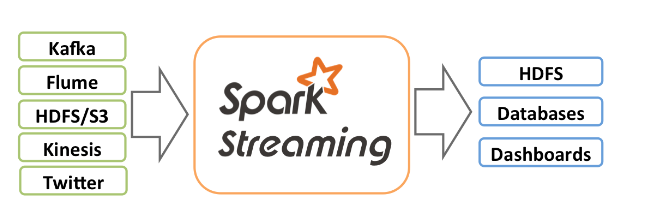
\includegraphics[scale=0.6]{spark_streaming}
	\end{center}
	\legend{Fonte: \citeauthor{sparkstreaming}, \citeyear{sparkstreaming}} 
\end{figure}

Para o \textit{streaming} de dados o Spark possui uma abstração chamada \textit{discretized stream} ou \textit{DStream}. \textit{DStream} podem ser criado a partir das fontes citados acima (kafka, Flume, etc.) ou qualquer outra fonte utilizando operacoes de alto nível. Internamente \textit{DStreams} são sequências de RDDs como demonstrado na figura~\ref{fig:sparkdstream}.

\begin{figure}[!h]
	\caption{\label{fig:sparkdstream} Representação de um \textit{DStream}.}
	\begin{center}
		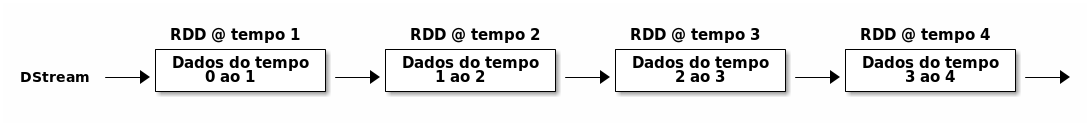
\includegraphics[scale=0.6]{spark_dstream}
	\end{center}
	\legend{Fonte: \citeauthor{sparkstreaming}, \citeyear{sparkstreaming}} 
\end{figure}
